Un médecin reçoit de nombreux patients. On dispose des informations suivantes :
\begin{itemize}
	\item 70\,\% des patients sont des enfants, les autres sont des adultes ;
	\item lorsque le patient est un enfant, le médecin prescrit des médicaments dans 20\,\% des cas ;
	\item lorsque le patient est un adulte, le médecin prescrit des médicaments dans 40\,\% des cas.
\end{itemize}

On choisit au hasard un patient reçu par ce médecin.

On considère les évènements suivants :
\begin{itemize}[left=5mm,label={}]
	\item $E$ : \og le patient est un enfant \fg{} ;
	\item $M$ : \og le médecin prescrit des médicaments \fg.
\end{itemize}

\begin{enumerate}
	\item Reproduire et compléter l'arbre pondéré ci-dessous.

	\begin{center}
		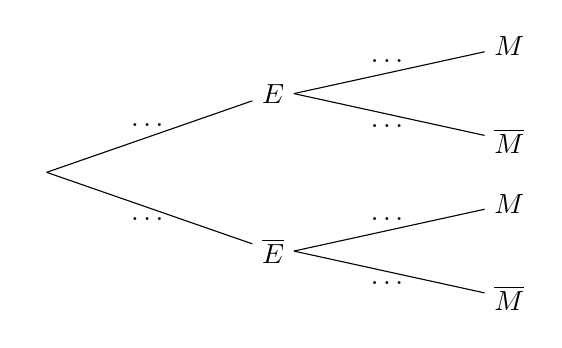
\begin{tikzpicture}[x=3cm, y=1cm]
			
			\node (root) at (0,0) {};
			\node (A) at (1,1) {$E$};
			\node (Abar) at (1,-1) {$\overline{E}$};
			\node (B1) at (2,1.6) {$M$};
			\node (B1b) at (2,0.4) {$\overline{M}$};
			\node (B2) at (2,-0.4) {$M$};
			\node (B2b) at (2,-1.6) {$\overline{M}$};
			
			\draw (root.east) -- (A) node[pos=0.5,above] {\ldots};
			\draw (root.east) -- (Abar) node[pos=0.5,below] {\ldots};
			
			\draw (A.east) -- (B1) node[pos=0.5,above] {\ldots};
			\draw (A.east) -- (B1b) node[pos=0.5,below] {\ldots};
			\draw (Abar.east) -- (B2) node[pos=0.5,above] {\ldots};
			\draw (Abar.east) -- (B2b) node[pos=0.5,below] {\ldots};
		\end{tikzpicture}
	\end{center}

	\item Calculer la probabilité $P\left(\overline{E} \cap M\right)$ et interpréter le résultat dans le contexte de l'exercice.
	\item Montrer que la probabilité que le médecin prescrive des médicaments au patient est égale à $0,26$.
	\item Les évènements $E$ et $M$ sont-ils indépendants ? Justifier.
	\item On sait que le médecin a prescrit des médicaments au patient.

	Quelle est la probabilité que le patient soit un enfant ? On donnera le résultat sous la forme d'une fraction irréductible.
\end{enumerate}
